\documentclass[11pt]{article}
\usepackage[margin=1in]{geometry}
\usepackage{amsmath, amssymb, amsthm}
\usepackage{enumitem}
\usepackage{xcolor}
\usepackage{indentfirst}
\usepackage{graphicx}
\usepackage{fancyhdr}
\usepackage{caption}
\usepackage{parskip}

\pagestyle{fancy}
\fancyhf{}
\rhead{Saha, Mishra}
\lhead{Algal Bloom in Lake Chapala}
\cfoot{\thepage}

\title{Algal Blooms in Lake Chapata: A Differential Equation Model}
\author{Soikat Saha\\Shruti D Mishra \\ \\
\small Math225: Differential Equations \\
\small Professor Cayce Fylling \\
\small Department of Mathematics, Gettysburg College}
\date{\today}

\begin{document}
% This is how you make a comment
\maketitle % This renders the title above, Edit title information in metadata above

\newpage

\tableofcontents % Automatically generates table of contents

\newpage

% Intro section starts
\section{Introduction}

\section*{This one with an asterisk does not}

\subsection{This subsection appears}

\subsection*{This one does not}

\subsubsection{Subsubsection}

% \begin{figure}
%     \centering
%     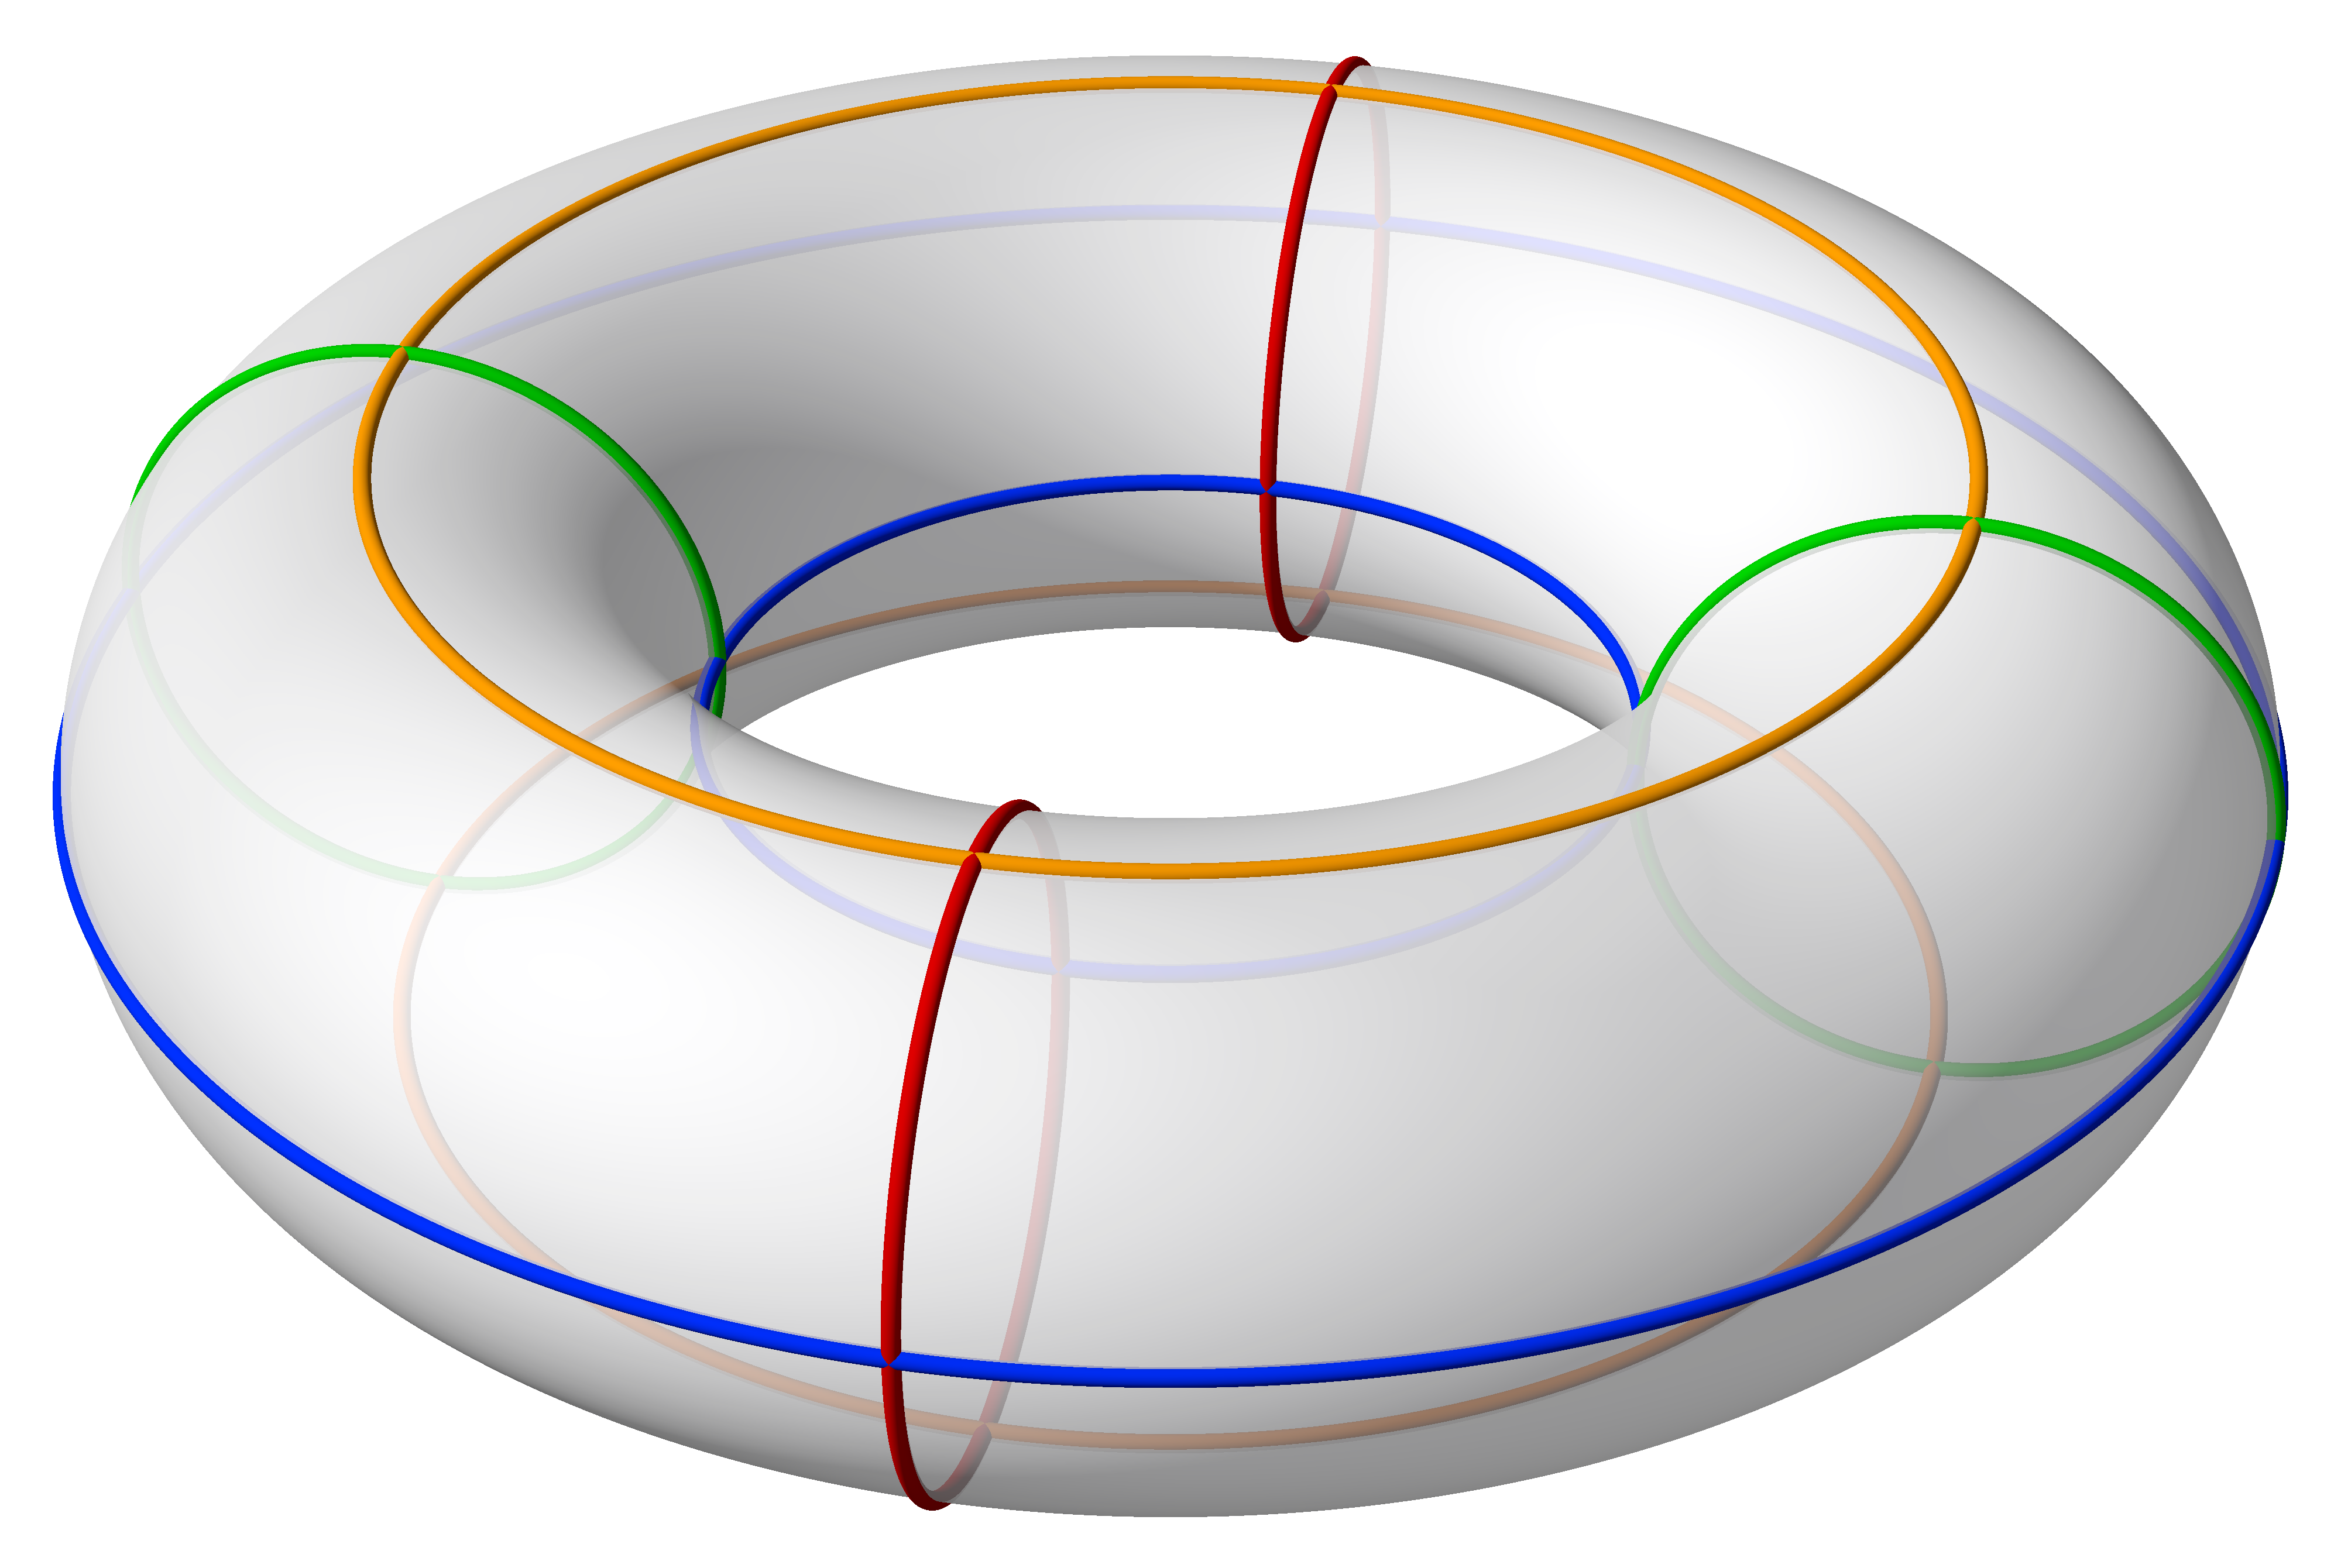
\includegraphics[width=0.5\linewidth]{Tesseract_torus.png}
%     \caption{This is a figure.}
%     \label{fig:figure_name}
% \end{figure}

I can reference the figure like this (\ref{fig:figure_name}).

I can also reference books or articles by adding them to my \texttt{biblio.bib} file and citing them like this \cite{key}.

\newpage

% Methods section starts
\section{Methods}

\subsection{Model development}

We kick off with an attempt to develop a resource-dependent model to describe the resilient ability of an algae population to bounce back after near-annihilation. To construct such a realistic model for algal blooms in Lake Chapada, we begin with the general structure 

\begin{equation}
    \frac{dy}{dt} = \text{Growth Function} - \text{Death Function}.
\end{equation}

Here, $y(t)$ represents the density of the algae population $(g/m^2)$, and $t$ represents time (days). Because the background suggests that chemical influx occurs periodically, we therefore seek to model using an oscillating function over time. 

\subsubsection{Model: V1}

To incorporate this periodic growth, the first model we consider is 

\begin{equation}
    \frac{dy}{dt} = -\cos{t}.
    \label{V1}
    \tag{V1}
\end{equation}

We plot this differential equation on a slope field plotter and observe the following characteristics of the general solution.

\begin{figure}[h]
    \centering
    
\includegraphics[width=0.65\linewidth]{figures/v1.png}
    \captionsetup{width=0.65\linewidth}
    \caption{Slope field for Differential Equation Model~\textbf{V1}, showing periodic oscillation in the rate of change.}
    \label{fig:fig-v1}
\end{figure}

As we can see in the slope field (Figure~\ref{fig:fig-v1}), this model represents an oscillating rate of change of population over time, varying between $-1$ and $+1$. The cosine function was chosen to reflect periodic growth and decline due to recurring agricultural chemical input. The derivatives, $-\cos{t}$, oscillates between $-1$ and $+1$, since
\[
    -1 \leq -\cos{t} \leq 1.
\]

However, this model poses several limitations and introduces scenarios that conflict with biological reality. To determine whether this oscillating growth rate also produces an oscillating population, we solve the differential equation model~\textbf{V1}:
\[
    \frac{dy}{dt} = -\cos t,
\]
\[
dy = -\cos t \, dt.
\]
Integrating, we get
\[
y(t) = -\sin t + C.
\]

Because $-\sin{t}$ oscillates between $-1$ and $+1$, the population exhibits oscillatory behavior. However, this model fails to address several important biological features and, in some cases predicts behavior that is clearly not biologically feasible.

First, at $t = 0$,
\[
    \frac{dy}{dt} = -\cos(0) = -1,
\]
so the model begins with negative growth. 

Second, the derivative does not depend on the population $y$. This implies that the same amount of growth or decline occurs regardless of whether the algae population is large or small. Biologically, this is unrealistic.

Most importantly, when the population reaches zero, the derivative may still be negative. This would cause the solution to move into negative population values, which are not biologically meaningful. Thus, model~\ref{V1} does not satisfy the requirement that the population remain nonnegative.

These limitations motivates us to modify the growth function to address the above concerns, ensure biological feasibility, and better represent realistic population dynamics.

\subsubsection{Model: V2}

To address the aforementioned limitations of the model~\ref{V1}, particularly the issue of negative growth at zero population and the lack of feasibility, we modify the oscillating growth function by shifting it upward. The revised model now becomes

\begin{equation}
    \frac{dy}{dt} = 1- \cos{t}
    \label{V2}
    \tag{V2}
\end{equation}

In this model, the cosine function is shifted upward by its amplitude which is 1. since $\cos{t}$ ranges between $-1$ and $+1$, the expression $1 - \cos t$ now ranges between $0$ and $2$. As a result, the rate of change is never negative.

This upward shift is helpful because it prevents the model from forcing the population to decrease when the population is already small. As observed in the model~\ref{V1}, the derivatives oscillated between $-1$ and $+1$, meaning the population could be pushed into negative values. In model~\ref{V2} however, the derivative is always nonnegative.

Below, we plot the differential equation model~\ref{V2} on a slope field plotter and look at its features.

\begin{figure}[h]
    \centering
    
\includegraphics[width=0.65\linewidth]{figures/v2.png}
    \captionsetup{width=0.65\linewidth}
    \caption{Slope field for model~\ref{V2}, showing the upward-shifted oscillating rate of change.}
    \label{fig:fig-v2}
\end{figure}

At $t = 0$,
\[
\frac{dy}{dt} = 1 - \cos(0) = 0,
\]
so the model begins with zero growth rather than negative growth, which resolves the negative population issue. Thus, shifting the oscillation upward ensures that growth remains biologically feasible and prevents the derivative from driving the population below zero.

However, although this modification improves feasibility, the derivatives still does not depend on the population $y$. This means the same amount of algae is added to the total population due to growth regardless of how large or small the population is, which, again, remains biologically unrealistic. Therefore, the model~\ref{V2} still lacks a mechanism that ties growth to the current population size.

\subsubsection{Model: V3}

Since model~\ref{V2} treated growth as a fixed amount added to the population, independent of the current population size, it remained biologically unrealistic. In real systems, population growth typically depends on how large the population already is. Therefore, to introduce dependency on the population, we modify the oscillating term from the previous model so that it acts as a growth rate rather than a fixed growth amount. The revised model is

\begin{equation}
    \frac{dy}{dt} = (1 - \cos{t})y
    \label{V3}
    \tag{V3}
\end{equation}

In this model, the oscillating term $1 - \cos t$ multiplies the population $y$, making the growth both time- and population-dependent. This means that when population is larger, the actual amount of growth is larger, and when the population is small, the amount of growth is proportionally smaller, which better reflects how growth occurs in real biological systems.

We plot the differential equation model~\ref{V2} on a slope field plotter below and observe how it changes $y$, population over $t$, time.

\begin{figure}[h]
    \centering
    
\includegraphics[width=0.65\linewidth]{figures/v3.png}
    \captionsetup{width=0.65\linewidth}
    \caption{Slope field for model~\ref{V3}, showing slopes that depend on both time and population size.}
    \label{fig:fig-v3}
\end{figure}

As observed in the slope field (Figure~\ref{fig:fig-v3}), model~\ref{V3} differs from model~\ref{V2} because the slopes now depend on both time and population size. In Version 2, slopes varied with time but remained the same vertically for all values of $y$. However, in Version 3, the slopes become steeper as $y$ increases and flatten near $y = 0$. This indicates that the population increases by a fraction of itself rather than by a fixed number. Thus, when the population is larger, it grows more rapidly, and when the population is smaller, it grows more slowly.

Biologically, this shows the difference between adding a constant number of algae each day (actual growth) and allowing the algae to grow at a fraction of its current total population (rate of growth).

Although, this model resolves several issue from previous models, it still lacks a way to represent removal or governmental intervention. Therefore, further refinement of the model remains necessary.

\subsubsection{Model: V4}

Although model~\ref{V3} incorporates growth more realistically by making it proportional to the population, it does not yet account for external intervention or removal. To represent consistent governmental efforts to reduce algae growth, we introduce a constant output term. The revised model is

\begin{equation}
    \frac{dy}{dt} = (1 - \cos{t})y - 1
    \label{V4}
    \tag{V4}
\end{equation}

Here, the newly introduced term $-1$ represents a constant removal of algae over time, independent of the current population size. Visually, this refined model preserves the periodic behavior of the population function while incorporating a constant death term. Compared to model~\ref{V3}, the population still grows periodically, but each cycle is reduced by a fixed amount due to the constant death function.

Below, we plot the model~\ref{V4} on a slope field plotter to visually observe the changes due to introducing the death function.

\begin{figure}[h]
    \centering
    
\includegraphics[width=0.65\linewidth]{figures/v4.png}
    \captionsetup{width=0.65\linewidth}
    \caption{Slope field for model~\ref{V4}, illustrating periodic growth with constant removal.}
    \label{fig:fig-v4}
\end{figure}

However, this assumption is also not biologically realistic. If the population becomes very small, removing the same fixed amount could drive the population below zero. In fact, if $y$ is sufficiently small, the constant removal term may outgrow the growth term, forcing the solution into negative values, near $y=0$.

Since population cannot be negative, this model may again violate feasibility. Therefore, although model~\ref{V4} introduces an important biological feature, government intervention, it does so in a way that is not entirely realistic. It is not feasible and often not realistic to assume that equal numbers of algae are continuously removed regardless of the population size. This leads us to modify the death function so that it becomes proportional to the population itself.





































I can reference the figure like this (\ref{fig:slopefield-v1}).

I can also reference books or articles by adding them to my \texttt{biblio.bib} file and citing them like this \cite{key}.


\bibliographystyle{plain}
\bibliography{biblio}

\end{document}